\documentclass[titlepage, a4paper]{article}
\usepackage[swedish]{babel}
\usepackage[utf8]{inputenc}
\usepackage{graphicx}
\usepackage{color}
\usepackage{mathtools}
\usepackage{etoolbox}
\usepackage{caption}
\usepackage{float}
\usepackage{listings}
% Sidformat
\usepackage{a4wide}
\usepackage[parfill]{parskip}
% Bättre bildtexter
\usepackage[margin=10pt,font=small,labelfont=bf,labelsep=endash]{caption}

% Enkelt kommando som låter mig attgöra-markera text
\newcommand{\todo}[1] {\textbf{\textcolor{red}{#1}}}

\usepackage{graphicx,epstopdf}
\usepackage{listings}
\epstopdfsetup{suffix=}
\DeclareGraphicsExtensions{.ps}
\DeclareGraphicsRule{.ps}{pdf}{.pdf}{`ps2pdf -dEPSCrop -dNOSAFER #1 \noexpand\OutputFile}

\lstset{literate=%
    {å}{{\r{a}}}1
    {ä}{{\"a}}1
    {ö}{{\"o}}1
    {Å}{{\r{A}}}1
    {Ä}{{\"A}}1
    {Ö}{{\"O}}1
}

%% Headers och Footers
\usepackage{fancyhdr}
\pagestyle{fancy}
\rhead{Martin Söderén \\ Alexander Yngve}
\chead{TANA21}

\begin{document}

{\ }\vspace{45mm}

\begin{center}
    \Huge \textbf{TANA21: Projektrapport}
\end{center}
\begin{center}
    \Large Integration
\end{center}

\vspace{250pt}

\begin{center}
    \begin{tabular}{|*{3}{p{40mm}|}}
        \hline
        \textbf{Namn} & \textbf{Personnummer} & \textbf{Epostaddress} \\ \hline
        {Martin Söderén} & {900929-1098} & {marso329@student.liu.se} \\ \hline
        {Alexander Yngve} & {930320-6651} & {aleyn573@student.liu.se} \\ \hline
    \end{tabular}
\end{center}
\newpage

\section{Inledning}
Denna rapport behandlar hur noggrann man kan integrera med hjälp av trapetsregeln samt den aritmetiska komplexiteten för integreringen.

\section{Uppgift}
Projektets uppgift är att skapa en MATLAB-funktion trapezoid som integrerar en funktion numeriskt med hjälp av trapetsregeln. Som argument tar funktionen in en funktion, startpunkt, slutpunkt och antalet delintervall.
\newline
\newline
Frågor att besvara:
\begin{itemize}
\item Är noggrannhetsordningen som förväntad?
\item Är den aritmetiska komplexiteten som förväntad?
\end{itemize}


\section{Teori}\label{sec:teori}
Den matematiska definitionen ser ut som följande och är tagen från kursboken avsnitt 7.2.
\begin{figure}[H]
  $$\int_a^b{f(x)dx=T(h)+R_T}$$
  
  $$ T(h)=h(\dfrac{1}{2}f_0+f_1+...+f_{n-1}+\dfrac{1}{2}f_n) $$
  Trunkeringsfelet ges av
  $$R_T=-\dfrac{b-a}{12}h^2f''(n) $$
  om $f''$ är kontinuerlig.
  \caption*{Definitionen av trapetsregeln från kursboken s.168}
\end{figure}

Det detta gör är en approximation av integralen genom att ställa upp en massa trapetser med bredd h under kurvan och summerar dessas areor. Se figur \ref{fig:trapets}.

\begin{figure}[H]
  \centering
  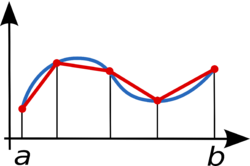
\includegraphics[scale=5.0]{trapets.png}
  \caption{Trapetsregeln}
  \label{fig:trapets}
\end{figure}

\section{Metod}\label{sec:metod}
Funktionerna implementerades enligt metoden beskriven i avsnitt 7.2 i kursboken. Därefter testades \textit{trapezoid} med koden i figur \ref{lst:test} och i figur \ref{lst:test2}. Det testkoden i figur \ref{lst:test2} gör är att för de testfunktionera som var givna i projektbeskrivningen integerera dessa med hjälp av \textit{trapezoid} och använda det analytiskt framtagna värden för integrationen och få fram felet. Dessa fel logaritmeras sedan och lutningen på kurvan används för att avgöra hur exakt trapetsmetoden är på funktionen.
\newline
\newline
Därefter testas tidskomplexiteten genom att uföra integereringar på $e^x$ med olika \textit{h} och mäta tiden det tar.

\section{Kod}
Funktionen \textit{trapezoid} (figur \ref{lst:trapezoid}) integrerar funktion f mellan a och b med hjälp av n stycken delintervall.

\begin{figure}[H]
  \begin{lstlisting}
function I =  trapezoid(f,a,b,n)
h=(b-a)/n;
I=(f(a)+f(b))/2;
for k=1:n-1
    I=I+f(a+k*h);
end
I=h*I;
end
  \end{lstlisting}
  \caption{\textit{trapezoid}}
  \label{lst:trapezoid}
\end{figure}


  \begin{lstlisting}

%test time complexity
n=[1 2 4 8 16 32 64 128 256 512 1024 2048 4096];
times=[];
for x=n
    tic;
trapets=trapezoid(@exp,0,1,x);
times=[times,toc];
end
plot(n,times);
xlabel('Intervals')
ylabel('Time')
  \end{lstlisting}
  \begin{figure}[H]
  \caption{Testkod för aritmetisk komplexitet}
  \label{lst:test}
\end{figure}


  \begin{lstlisting}
n=[1 2 4 8 16 32 64 128 256 512 1024 2048 4096];
data=zeros(7,length(n));
i=1;
for x=n
    %e^x [0 1]
    data(1,i)=abs((exp(1)-exp(0))-trapezoid(@exp,0,1,n(i)));
    
    %3*x^2+2*x+1 [0 1]
    f=@(x) 3*x^2+2*x+1;
    f_int=@(x) x^3+x^2+x;
    data(2,i)=abs((f_int(1)-f_int(0))-trapezoid(f,0,1,n(i)));
    
    %2*x+2 [0 1]
    f=@(x) 2*x+2;
    f_int=@(x) x^2+2*x;
    data(3,i)=abs((f_int(1)-f_int(0))-trapezoid(f,0,1,n(i)));
    
    %5*x^4+3*x^3+4*x^2+x+15 [0 1]
    f=@(x) 5*x^4+3*x^3+4*x^2+x+15;
    f_int=@(x) x^5+(3/4)*x^4+(4/3)*x^3+(1/2)*x^2+15*x;
    data(4,i)=abs((f_int(1)-f_int(0))-trapezoid(f,0,1,n(i)));
    
    %4/(1+x^2) [0 1]
    f=@(x) 4/(1+x^2);
    data(5,i)=(4*(atan(1)-atan(0)))-trapezoid(f,0,1,n(i));

    %x^(1/2) [0 1]
    f=@(x) x^(1/2);
    f_int=@(x) (2/3)*x^(3/2);
    data(6,i)=abs((f_int(1)-f_int(0))-trapezoid(f,0,1,n(i)));

    %sin(x) [0 2*pi]    
    f=@(x) sin(x);
    f_int=@(x) -cos(x);
    data(7,i)=abs((f_int(2*pi)-f_int(0))-trapezoid(f,0,2*pi,n(i)));
    
    i=i+1;
end
clf
hold on;
for j=[1:1:6]
plot(log(n),log(data(j,:)))
log_data=log(data(j,:));
log_axis=log(n);
(log_data(length(data(j,:)))-log_data(1))/(log_axis(length(log_axis))-log_axis(1))
end
xlabel('log(h)')
ylabel('log(error)')
legend('e^x','3*x^2+2*x+1', '2*x+2','5*x^4+3*x^3+4*x^2+x+15','4/(1+x^2)','x^{1/2}')

data;
  \end{lstlisting}
  \begin{figure}[H]
  \caption{Testkod för felen}
  \label{lst:test2}
\end{figure}

\section{Validering}
För samtliga funktioner i testkoden så togs en analytiskt integration fram som användes till referens vid testen. Inget fel var större än $10^{-5}$ vilket gör att man kan anta att funktionen räknar rätt. Samliga fel för alla funktioner återfinns under resultat.

\section{Resultat}
Resultatet av testet beskrivet i avsnitt \ref{sec:metod} återges i tabell \ref{tab:resultat}.

\begin{table}[H]
  \centering
  \begin{tabular}{|l|l|}
    \hline
    \textbf{Funktion [gränser]} & \textbf{Noggrannhetsordning} \\ \hline
    $e^x \quad [0 \ 1]$ & 2 \\ \hline
    $3x^2+2x+1$ \quad [0 \ 1] & 2 \\ \hline
    $2x+2$ \quad [0 \ 1] & 0 \\ \hline
    $5x^4+3x^3+4x^2+x+15$ \quad [0 \ 1] & 2 \\ \hline
    $4/(1+x^2)$ \quad [0 \ 1] & 2\\ \hline
    $x^{(1/2)}$ \quad [0 \ 1] & 1.5 \\ \hline
    $sin(x)$ \quad [0 \ $2\pi$] & 0 \\ \hline
  \end{tabular}
  \caption{Resultat för de olika funktionernas noggrannhetsordning}
  \label{tab:resultat}
\end{table}

\begin{figure}[H]
  \centering
  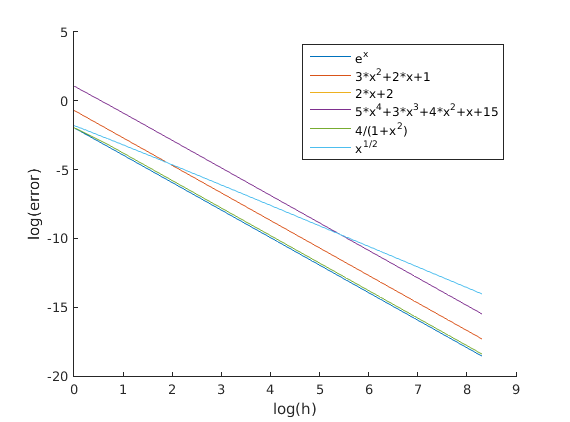
\includegraphics[scale=0.8]{errors2.png}
  \caption{Felet vid olika antal intervall.}
  \label{fig:intervalls}
\end{figure}

Från figur \ref{fig:intervalls} kan man urskilja att felet avtar snabbt då \textit{h} ökar. Resultatet i tabell~\ref{tab:resultat} togs fram genom lutningen på varje funktions linje i figur ~\ref{fig:intervalls}. $sin(x)$ är inte med i figuren då dess fel var $\approx 0$ vilket gav en konstig linje. Anledningen till att $sin(x)$:s fel var noll beror på att den är periodisk. $2x+2$:s fel var också noll och detta beror på att dess andraderivata är noll och att dess integral blir väldigt exakt om approximerar den med trapetsmetoden. 

\begin{figure}[H]
  \centering
  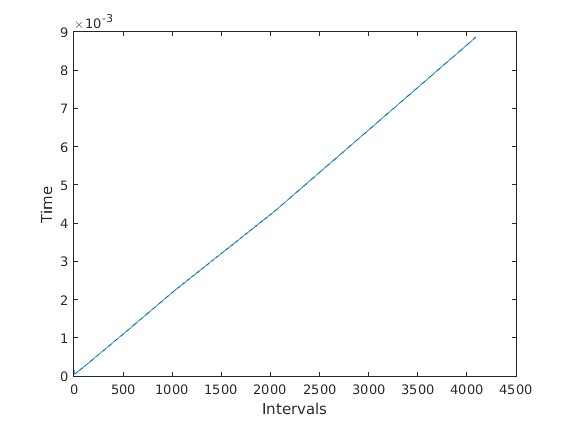
\includegraphics[scale=0.6]{time.png}
  \caption{Tiden vid olika antal intervall.}
  \label{fig:time}
\end{figure}
Från figur \ref{fig:time} kan man se att tidskomplexiteten är linjärt beroende av antalet intervall man använder eller längden \textit{h} på alla trapetser. Detta är rimligt med hänsyn på definitionen då ett extra intervall ger en extra term att addera.


\section{Diskussion}
Noggranhetsordningen är som förväntat på två. Det vill säga den dominerande feltermen är proportionell mot $h^2$. Den aritmetiska tidskomplexiteten är linjär mot h det vill säga den är $\mathcal{O}(n)$, vilket är som förväntat.
\end{document}

